%	!Mode::"UTF-8"
%	本模板设置改自北京大学交叉学院 王宇哲学长和北京大学化学与分子工程学院 王应泽同学的分享,特此感谢!
%	模板制作:北京大学化学与分子工程学院 王梓涵
%	Email:2100011837@stu.pku.edu.cn
%	本模板仅适用于北京大学物理化学实验报告,其他学校请自行修改
%	吐槽:Latex用于写物化实验报告还是过于繁琐了,不过还是比Word好用多了(๑•̀ㅂ•́)و✧ (此吐槽由copilot自动生成,模板作者认为word更好用)
%	本模板仅供交流学习使用,不可用作商业用途。

\documentclass[12pt]{article}

%	页面设置
\usepackage{geometry}
\geometry{left=2.5cm, right=2.5cm, top=2.5cm, bottom=2.5cm}
\usepackage{graphicx}
\usepackage{ctex}
\usepackage{fontspec}
\usepackage{setspace}
\usepackage[usenames,dvipsnames]{xcolor}
\usepackage{titlesec}

%	字体设置
\setmainfont{Times New Roman}
\setCJKmainfont{SimSun}
\setCJKsansfont{SimHei}
\setCJKmainfont[AutoFakeBold=true]{SimSun}

%	表格设置\
\usepackage{array,colortbl}
\usepackage{makecell}
\newcommand{\addcell}[2][4]{\makecell{\zihao{#1}\textsf{#2}}}
\usepackage{titlesec}
\usepackage{booktabs}
\usepackage{ragged2e} 
\usepackage{multirow}
\usepackage{tabularx}

% 网址设置
\usepackage{hyperref}
\hypersetup{hidelinks,
	colorlinks=true,
	allcolors=black,
	pdfstartview=Fit,
	breaklinks=true}


%	设置图注、表注
\usepackage{caption}
\usepackage{bicaption}
\captionsetup{labelsep=quad, font={small, bf}, skip=2pt}
\DeclareCaptionOption{english}[]{
    \renewcommand\figurename{Fig.}
    \renewcommand\tablename{Table}
}
\captionsetup[bi-second]{english}

%	设置页眉
\usepackage{fancyhdr}
\usepackage{xpatch}
\pagestyle{fancy}
\fancypagestyle{preContent}{
    	\fancyhead[L]{\zihao{-5} 物理化学实验}
    	\fancyhead[C]{\zihao{-5} 实验六\ \ 溶液表面吸附的测定}
    	\fancyhead[R]{\zihao{-5} 2100011837\ 王梓涵}
		\renewcommand{\headrulewidth}{2pt}
		\renewcommand{\footrulewidth}{1pt}
		\xpretocmd\headrule{\color{BrickRed}}{}{\PatchFailed} % 设置页眉分割线颜色
		\xpretocmd\footrule{\color{BrickRed}}{}{\PatchFailed} % 设置页脚分割线颜色
}
\pagestyle{preContent}



%	设置首页页眉及取消首页页脚 若不需要首页页眉 请注释掉下列内容
\fancypagestyle{plain}{
	\fancyhead[L]{\zihao{-5} 物理化学实验}
    \fancyhead[C]{\zihao{-5} 实验六\ \ 溶液表面吸附的测定}
	\fancyhead[R]{\zihao{-5} 2100011837\ 王梓涵}
	\cfoot{}
}

%	设置标题格式
\titleformat*{\section}{\color{Mahogany}\zihao{4}\sffamily}
\titleformat*{\subsection}{\zihao{-4}\sffamily}
\titleformat*{\subsubsection}{\zihao{-4}\sffamily}
\titlespacing*{\section}{0pt}{10pt}{10pt}
\titlespacing*{\subsection}{0pt}{10pt}{5pt}
\titlespacing*{\subsubsection}{0pt}{10pt}{5pt}


%	设置引用格式(ACS格式规范)
%	注意:请安装JabRef
%	JabRef使用参考:https://blog.csdn.net/weixin_44191286/article/details/85698921
\usepackage[super,round,comma,compress]{natbib}

%	数学公式增强
\usepackage{amsmath}
\usepackage{amssymb}

%	单位与数学式
\usepackage{siunitx}

% 其他添加
\usepackage[version=4]{mhchem}

%	设置封面
\begin{document}
    % 标题页
    \begin{titlepage}
    	% 页眉
    	\thispagestyle{plain}
        % 校徽图片
        \begin{figure}[h]
            \centering
            \includegraphics{pku.png}
        \end{figure}
        \vspace{24pt}
        % 标题
        \centerline{\zihao{-0} \textsf{\textcolor{Mahogany}{物理化学实验报告}}}
        \vspace{40pt} % 空行
        \begin{center}
            \begin{tabular}{cp{14.1cm}}
                % 题目
                \addcell[2]{题目:} & \addcell[1]{溶液表面吸附的测定} \\
                \cline{2-2}
            \end{tabular}
        \end{center}
        \vspace{20pt} % 空行
        \begin{center}
            \doublespacing
            \begin{tabular}{cp{5cm}}
                % 姓名
                \addcell{姓\phantom{空格}名:\ } & \addcell{王梓涵} \\
                \cline{2-2}
                % 学号
                \addcell{学\phantom{空格}号:\ } & \addcell{2100011837}\\
                \cline{2-2}
                % 组别
                \addcell{组\phantom{空格}别:\ } & \addcell{22组} \\
                \cline{2-2}
                % 实验日期
                \addcell{实验日期:\ } & \addcell{2023.11.02}\\
                \cline{2-2}
                % 室温
                \addcell{室\phantom{空格}温:\ } & \addcell{295.65\ K}\\
                \cline{2-2}
                % 大气压强
                \addcell{大气压强:\ } & \addcell{99.89\ kPa}\\
                \cline{2-2}
            \end{tabular}
            \begin{tabular*}{\textwidth}{c}
                \\ % 这是空行
                \\ % 这是空行
                \\ % 这是空行
                \hline % 分割线
            \end{tabular*}
        \end{center}
        % 摘要
        \textsf{\textcolor{BrickRed}{摘\ \ 要}}\ \  \  本实验利用最大气泡压力法和吊片法,对去离子水和8个不同浓度正丁醇溶液的表面张力进行了测定,作出了正丁醇水溶液的$\gamma-{\rm ln}c$等温曲线。最大气泡压力法计算得正丁醇分子的饱和吸附量$\Gamma_{\infty}=(5.52\pm 0.12)\times 10^{-6}\ \ {\rm mol\cdot m^{-2}}$、饱和吸附下每个正丁醇分子占有的表面积$q=(0.301\pm 0.064)\ \ {\rm nm^{2}}$。当正丁醇浓度$c=0.740\ \ {\rm mol\cdot L^{-1}}$时,每个分子实际占据的面积$q_{c}=(0.26\pm 0.05)\ \ {\rm nm^{2}}$。通过吊片法计算得$\Gamma_{\infty}=(5.402\pm 0.04)\times10^{-6}\ \ {\rm mol\cdot m^{-2}}$,$q=0.307\ \ {\rm nm^{2}}$,$c=0.740\ \ {\rm mol\cdot L^{-1}}$时$q_{c}=(0.26\pm 0.002)\ \ {\rm nm^{2}}$。
        \\
        \\
        % 关键字
        \textsf{\textcolor{BrickRed}{关键词}}\ \ 最大气泡压力法;吊片法;表面张力;饱和吸附
    \end{titlepage}

    \section{引言}
		\subsection{实验目的}
			本实验的实验目的主要有以下几点\citealp{physchemlab}:\par
			\ \ \ \ \ \ \ \ 1. 掌握计算溶液表面吸附量和每个分子占据表面积的方法。\par
			\ \ \ \ \ \ \ \	2. 掌握最大气泡法和吊片法测量表面张力。\par
			\ \ \ \ \ \ \ \	3. 了解气泡压力与半径以及表面张力的关系。\par
			\ \ \ \ \ \ \ \	4. 了解不同测量表面张力的方法的区别。\par

		\par
			\subsection{实验原理和实验方法}
				实验原理和实验方法在实验预习报告中如\textbf{图1}所示: \par
		\begin{figure}[h]
			\centering
			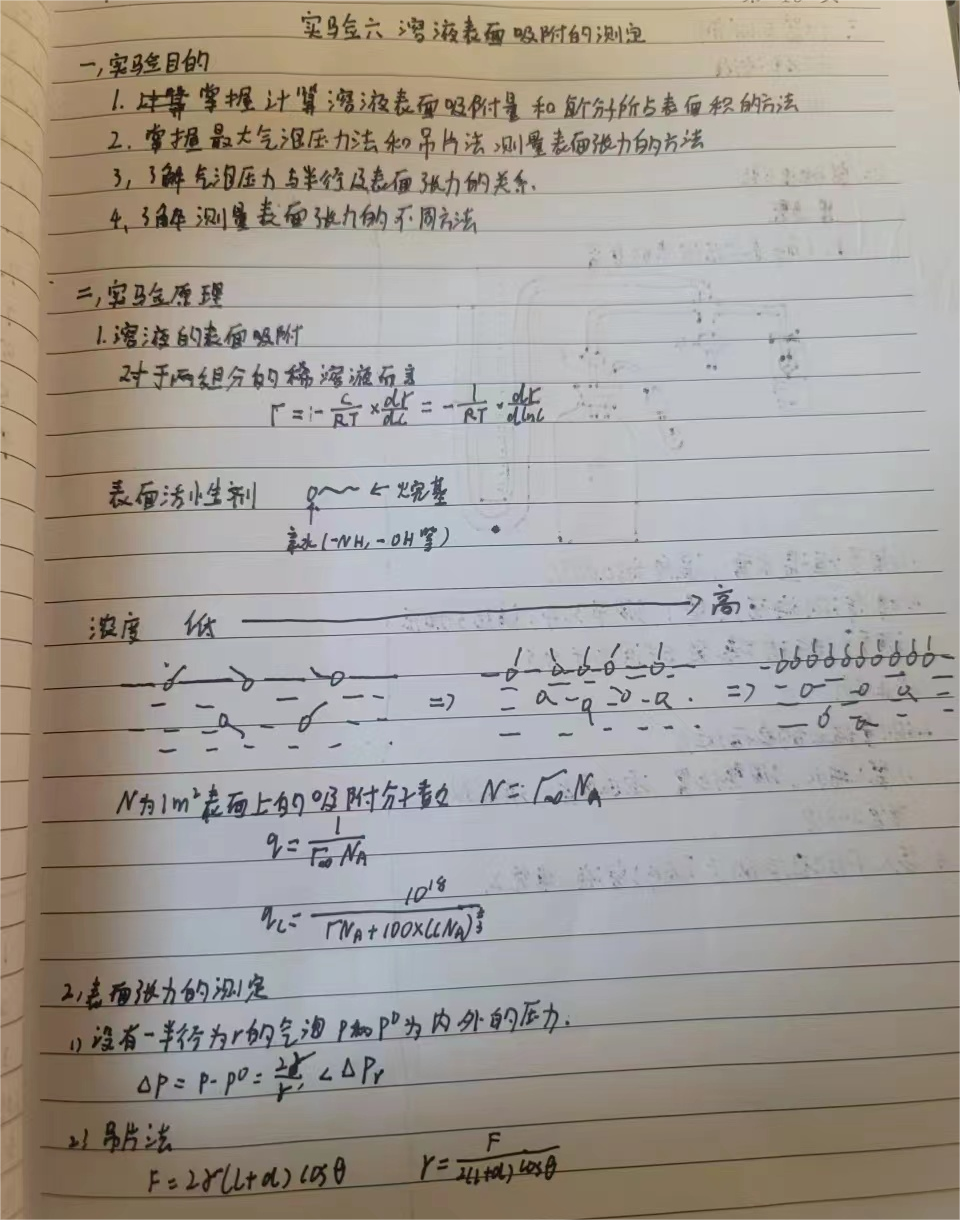
\includegraphics[width=0.65\textwidth]{1.png}
			\bicaption{实验预习报告的实验原理部分}{The principle part of the experiment in the experiment preview report}
		\end{figure}

	     
    \section{实验部分}

    	\subsection{仪器和试剂}
		\textbf{仪器}:\ \  最大气泡压力法表面张力测定装置(如\textbf{图2}所示),QBZY-2型表面张力仪,恒温水浴装置。\par
		\textbf{试剂}:\ \  纯水,$8$种不同浓度的正丁醇溶液(浓度分别为$0.0218\ \ {\rm M}$、$0.0547\ \ {\rm M}$、$0.111\ \ {\rm M}$、$0.220\ \ {\rm M}$、$0.329\ \ {\rm M}$、$0.439\ \ {\rm M}$、$0.550\ \ {\rm M}$、$0.740\ \ {\rm M}$)。
			
			\begin{figure}[h]
				\centering
				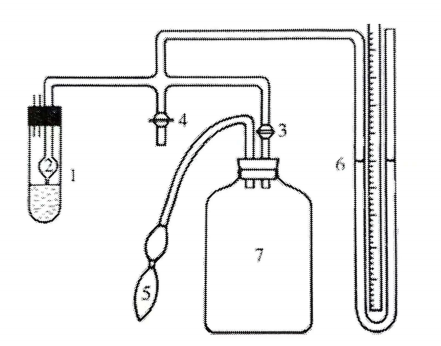
\includegraphics[width=0.70\textwidth]{2.png}
				\bicaption{最大气泡压力法仪器图}{Maximum bubble pressure method instrument diagram}
			\end{figure}

    	 \subsection{实验内容\citealp{physchemlab}}
			\subsubsection{最大气泡压力法测量纯水表面张力}
			调节恒温槽,将温度设定为$30.00\ \ {\rm ^{\circ}C}$。检查并使用洗耳球清洗毛细管,将约$2 \ \ {\rm mL}$纯水装入试管\textbf{1},调整好毛细管\textbf{2}的位置,使毛细管尖端与溶液液面相切。\par 
			打开安全阀\textbf{4},关闭调节活塞\textbf{3},记录无压力时压力计左右两管液柱高度$h_{L}$、$h_{R}$及液柱高度差$\Delta h_{0}=h_{R}-h_{L}$,重复读取3次,取平均值作为压力计的零点位置。\par 
			关闭活塞和安全阀,通过双联球给缓冲瓶加压。小心调节活塞的针阀(\textbf{一定要小心,不然会将U型管中的水喷出来。若喷出来则需重新调节记录零点}),使气泡从产生到爆裂的时间大于$8\ \ {\rm s}$。当气泡逸出毛细管尖端时,压力计的水柱差会突然下降,记录下降前的水柱最大高度差$\Delta h$,重复4次,计算$\Delta h$的平均值。
			\subsubsection{最大气泡压力法测量正丁醇表面张力}
			检查并清洗毛细管,依次测量8个不同浓度的正丁醇溶液的压力差值,每次测量前用下一次的正丁醇溶液润洗毛细管内壁和试管$2\sim 3$次,用同法依次测定8个不同浓度的正丁醇溶液的左右液面高度。
				
			\subsubsection{吊片法测量表面张力}
			1.接通QBZY-2型表面张力仪电源,挂上吊钩,按“开/关”键,预热30\ \ min。\par
			2.按“手动/自动”键,将仪器调至自动状态。\par
			3.用镊子夹取白金板,用去离子水清洗(\textbf{其实没必要,灼烧即可去掉所有有机物溶液}),随后用酒精灯灼烧白金板,保持白金板与水平面呈$45^{\circ}$角进行,直至白金板变红,将白金板挂在挂钩上冷却。\par 
			4.将待测溶液加入样品皿中,置于升降样品台上并将处理好并已经冷却的白金板挂在吊钩上。\par
			5.按“去皮”键作清零处理,按“向上”键开始表面张力的自动测定,待显示屏数值稳定后(\textbf{除纯水外,数值并不会真的到达稳定,这部分的原因会在实验讨论部分讨论}),读取相应的表面张力$\gamma$。\par
			6.测量完成后,按“向下”键将样品与白金板脱离。\par
			整组重复第$3\sim6$步完成对8个不同浓度正丁醇溶液的测量(各测1次),汇总实验数据。实验结束后将白金板灼烧、样品皿洗净,关机。

     \vbox{}
	 \section{数据与结果}
 		\subsection{实验数据处理}
 			\subsubsection{最大气泡压力法零点位置测量}
			按照\textbf{2.2.1}中的步骤首先读取无压力时压力计左右两管液柱高度$h_{L}$、$h_{R}$及液柱高度差$\Delta h_{0}=h_{R}-h_{L}$,即压力计无压力时的零点位置,结果示于\textbf{表1}。
			\begin{table}[h]
				\arrayrulecolor{Maroon}
				\centering
				\zihao{5}
				\bicaption{压力计零点位置测量数据}{Pressure gauge zero position measurement data}
				\begin{tabular}{cccc}
					\toprule
					编号 & $h_{L}/{\rm cm}$ & $h_{R}/{\rm cm}$ & $\Delta h_{0}/{\rm cm}$ \\
					\midrule
					1 & 23.95 & 23.95 & 0.00\\
					2 & 23.92 & 24.00 & 0.08\\
					3 & 23.94 & 23.98 & 0.04\\
					4 & 23.95 & 23.96 & 0.01\\
					\bottomrule
				\end{tabular}
			\end{table}
			\par
			根据\textbf{表1}数据,计算$\Delta h_{0}$的平均值为:
				$$
				\Delta h_{0}=0.03\ {\rm cm}
				$$
			$\Delta h_{0}$的标准偏差为:
				$$
				\sigma_{\Delta h_{0}}=\sqrt{\frac{0.00^{2}+0.08^{2}+0.04^{2}+0.01^{2}}{4-1}}=0.04\ {\rm cm}
				$$
			\subsubsection{最大气泡压力法测量纯水表面张力}
			调节活塞的针阀,通过最大气泡压力法测量纯水的表面张力,记录压力计左右两管液柱高度$h_{L}$、$h_{R}$。(\textbf{但在实际测量过程中,气泡的破裂会立即减少液面高度差,实验人员并来不及记录左右两个高度,所以实际上实验仅记录了$h_{R}$,$h_{L}$是通过$h_{L}=h_{L,0}-(h_{R}-h_{R,0})$间接得到,这部分造成的误差会在实验讨论部分讨论。})各项测量数据示于\textbf{表2}:\par
			\begin{table}[h]
				\arrayrulecolor{Maroon}
				\centering
				\zihao{5}
				\bicaption{最大气泡压力法测量纯水表面张力数据}{Measurement data of surface tension of water via maximum bubble pressure method}
				\begin{tabular}{cccc}
					\toprule
					编号 & $h_{L}/{\rm cm}$ & $h_{R}/{\rm cm}$ & $\Delta h^{\prime}/{\rm cm}$ \\
					\midrule
					1 & 19.64 & 28.28 & 8.56 \\
					2 & 19.65 & 28.27 & 8.54\\
					3 & 19.64 & 28.28 & 8.56\\
					4 & 19.64 & 28.28 & 8.56\\
					\bottomrule
				\end{tabular}
			\end{table}
			计算$\Delta h^{\prime}$的平均值为:
				$$
				\Delta h^{\prime}=8.55\ {\rm cm}
				$$
			$\Delta h^{\prime}$的标准偏差为:
				$$
				\sigma_{\Delta h^{\prime}}=\sqrt{\frac{0.01^{2}+0.02^{2}+0.01^{2}+0.01^{2}}{4-1}}=0.01\ {\rm cm}
				$$
			考虑到压力计零点修正,计算实际的液柱高度差为:
				$$
				\Delta h=\Delta h^{\prime}-\Delta h_{0}=8.52\ {\rm cm}
				$$
			故实际的液柱高度差为:
				$$
				\Delta h=(8.52\pm 0.01)\ {\rm cm}
				$$
			
			\subsubsection{最大气泡压力法测量正丁醇表面张力}
			与测量纯水表面张力的步骤相同,每次测量前需用新的溶液将毛细管内壁和试管洗涤$2\sim 3$次,通过最大气泡压力法测量8个不同浓度正丁醇溶液的表面张力,其中$\Delta h/{\rm cm}$为考虑零点修正后的结果,即:
			$$
			\Delta h=\Delta h^{\prime}-\Delta h_{0}
			$$
 			各项测量数据示于\textbf{表3}:\par
			\begin{table}[h]
				\arrayrulecolor{Maroon}
				\centering
				\zihao{5}
				\bicaption{最大气泡压力法测量正丁醇表面张力数据}{Measurement data of surface tension of n-BuOH via maximum bubble pressure method}
				\begin{tabular}{cccccc}
					\toprule
					$c_{\rm BuOH}/{\rm mol\cdot L^{-1}}$ & 编号 & $h_{L}/{\rm cm}$ & $h_{R}/{\rm cm}$ & $\Delta h_{0}$ or $\Delta h^{\prime}/{\rm cm}$ & $\Delta h/{\rm cm}$  \\
					\midrule
		   ~      & 1  &19.91 & 28.03 & 8.06 & ~ \\
		   0.0218 & 2  &19.91 & 28.03 & 8.06 & 8.04$\pm$0.01 \\
		   ~      & 3  &19.91 & 28.03 & 8.06 & \\
		   		  & 4  &19.90 & 28.04 & 8.08 & \\
					\midrule
		   ~      & 1  &20.23 & 27.67 & 7.44 & ~ \\
		   0.0547 & 2  &20.22 & 27.68 & 7.46 & 7.45$\pm$0.01\\
		   ~      & 3  &20.23 & 27.67 & 7.44 & \\
		   		  & 4  &20.22 & 27.68 & 7.46 & \\
		   \midrule
		   ~      & 1  &20.73 & 27.19 & 6.42 & ~ \\
		   0.111  & 2  &20.74 & 27.18 & 6.40 & 6.39$\pm$0.03\\
		   ~      & 3  &20.71 & 27.21 & 6.46 & ~ \\
		   		  & 4  &20.72 & 27.20 & 6.44 & ~ \\
		   \midrule
		   ~      & 1  &21.25 & 26.65 & 5.40 & ~ \\
		   0.220  & 2  &21.25 & 26.65 & 5.40 & 5.40$\pm$0.00\\
		   ~      & 3  &21.25 & 26.65 & 5.40 & ~ \\
		   		  & 4  &21.25 & 26.65 & 5.40 & ~ \\
		   \midrule
		   ~      & 1  &21.59 & 26.33 & 4.56 & ~ \\
		   0.329  & 2  &21.60 & 26.32 & 4.54 & 4.68$\pm$0.01\\
		   ~      & 3  &21.59 & 26.33 & 4.56 & \\
		   		  & 4  &21.59 & 26.33 & 4.56 & \\
		   \midrule
		   ~      & 1  &21.78 & 26.12 & 4.34 & ~ \\
		   0.439  & 2  &21.79 & 26.11 & 4.32 & 4.32$\pm$0.02\\
		   ~      & 3  &21.80 & 26.10 & 4.30 & \\
		   		  & 4  &21.79 & 26.11 & 4.32 & \\
		   \midrule
		   ~      & 1  &22.09 & 25.82 & 3.72 & ~ \\
		   0.550  & 2  &22.10 & 25.81 & 3.70 & 3.71$\pm$0.02\\
		   ~      & 3  &22.07 & 25.84 & 3.76 & \\
		   		  & 4  &22.09 & 25.82 & 3.72 & \\
		   \midrule
		   ~      & 1  &22.20 & 25.70 & 3.44 & ~ \\
		   0.740  & 2  &22.20 & 25.70 & 3.44 & 3.38$\pm$0.01\\
		   ~      & 3  &22.20 & 25.70 & 3.44 & \\
		   		  & 4  &22.20 & 25.70 & 3.44 & \\
					\bottomrule
				\end{tabular}
			\end{table}
		   \par 
		\subsubsection{吊片法测量表面张力}
		用吊片法依次测量纯水和8个不同浓度的正丁醇溶液的表面张力。整组共同完成对8个不同浓度正丁醇溶液的测量(各测1次),汇总各项数据示于\textbf{表4}。
		\begin{table}[h]
			\arrayrulecolor{Maroon}
			\centering
			\zihao{5}
			\bicaption{吊片法测量表面张力数据}{Measurement data of surface tension via pendant drop method}
			\begin{tabular}{cccccccccc}
				\toprule
				$c_{\rm BuOH}/{\rm mol\cdot L^{-1}}$  	& 0		& 0.0218& 0.0547& 0.111& 0.220& 0.329& 0.439& 0.550& 0.740\\
				\midrule
				$\gamma/{\rm mN\cdot m^{-1}}$ 			& 71.30 & 66.24 & 60.94 & 55.20& 47.52& 42.24& 38.43& 35.54& 31.40\\
				\bottomrule
			\end{tabular}
		\end{table}

		\subsection{数据处理结果与分析}
			\subsubsection{大气泡压力法计算各浓度正丁醇水溶液的$\gamma$值}
			根据最大气泡压力法的实验原理,溶液表面张力$\gamma$与压力计左右两管液柱高度差$\Delta h$成正比。记纯水的表面张力为$\gamma_{\rm H_{2}O}$,纯水对应的压力计左右两管液柱高度差为$\Delta h_{\rm H_{2}O}$,则有:\par
			$$
			\gamma=\frac{\gamma_{\rm H_{2}O} \Delta h}{\Delta h_{\rm H_{2}O}}
			$$
			\par
			查阅手册\citealp{crc}得$30\ \ {\rm ^{\circ }C}$以下纯水的表面张力$\gamma_{\rm H_{2}O}=71.20\ \ {\rm mN\cdot m^{-1}=0.07120\ \ {\rm J\cdot m^{-2}}}$,实验测得对应的液柱高度差$\Delta h_{\rm H_{2}O}=8.53\ \ {\rm cm}$,对于各浓度正丁醇水溶液,将上述数据及实验测得的液柱高度差$\Delta h$代入公式中,即可计算得到各浓度正丁醇水溶液的表面张力$\gamma$。\par 
			对于标准差$\sigma_{\gamma}$,以第一组$c_{\rm BuOH}= 0.0218{\rm mol\cdot L^{-1}}$为例$\sigma_{\Delta h}=0.01\ \ {\rm cm}$,$\sigma_{\Delta h_{\rm H_{2}O}}=0.01\ \ {\rm cm}$此时:
			$$
			\sigma_{\gamma}=\frac{\gamma_{\rm H_{2}O}}{\Delta h_{\rm H_{2}O}}\sqrt{\sigma_{\Delta h}^{2}+(\frac{\Delta h}{\Delta h_{\rm H_{2}O}} \sigma_{\Delta h_{\rm H_{2}O}})^{2}}=0.00011\ \ {\rm J\cdot m^{-2}}
			$$
			各浓度正丁醇水溶液的表面张力$\gamma$计算结果示于\textbf{表5}。\par
			\begin{table}[h]
				\centering
				\zihao{5}
				\bicaption{不同浓度正丁醇水溶液表面张力$\gamma$计算结果}{Calculation results of $\gamma$ of n-BuOH aqueous solution}
				\begin{tabular}{cccc}
					\toprule
					$c_{\rm BuOH}/{\rm mol\cdot L^{-1}}$ & $\Delta h / {\rm cm}$ &$\sigma_{\Delta h}/{\rm cm}$& $\gamma/{\rm J\cdot m^{-2}}$\\
					\midrule
					0.0218 & 8.04& 0.01 &0.06711$\pm$0.00011 \\
					0.0547 & 7.45& 0.01&0.06218$\pm$0.00011\\
					0.111 & 6.39 & 0.03 &0.05334$\pm$0.00026\\
					0.220 & 5.40 & 0.00 &0.04507$\pm$0.00005\\
					0.329 & 4.68 & 0.01 &0.03906$\pm$0.00009\\
					0.439 & 4.32 & 0.02 &0.03606$\pm$0.00017\\
					0.550 & 3.71 & 0.02 &0.03098$\pm$0.00017\\
					0.740 & 3.38 & 0.01 &0.02821$\pm$0.00008\\
					\bottomrule
				\end{tabular}
			\end{table}
					
			\subsubsection{正丁醇水溶液$\gamma-{\rm ln}c$等温曲线与饱和吸附量$\Gamma_{\infty}$}
			根据\textbf{2.2.2}中的实验原理,正丁醇水溶液的表面张力$\gamma$与正丁醇的浓度$c$成负指数关系,即$\gamma$与${\rm ln}c$成线性关系,故作出正丁醇水溶液的$\gamma-{\rm ln}c$等温曲线,如\textbf{图3}所示。
			\begin{figure}[h]
				\centering
				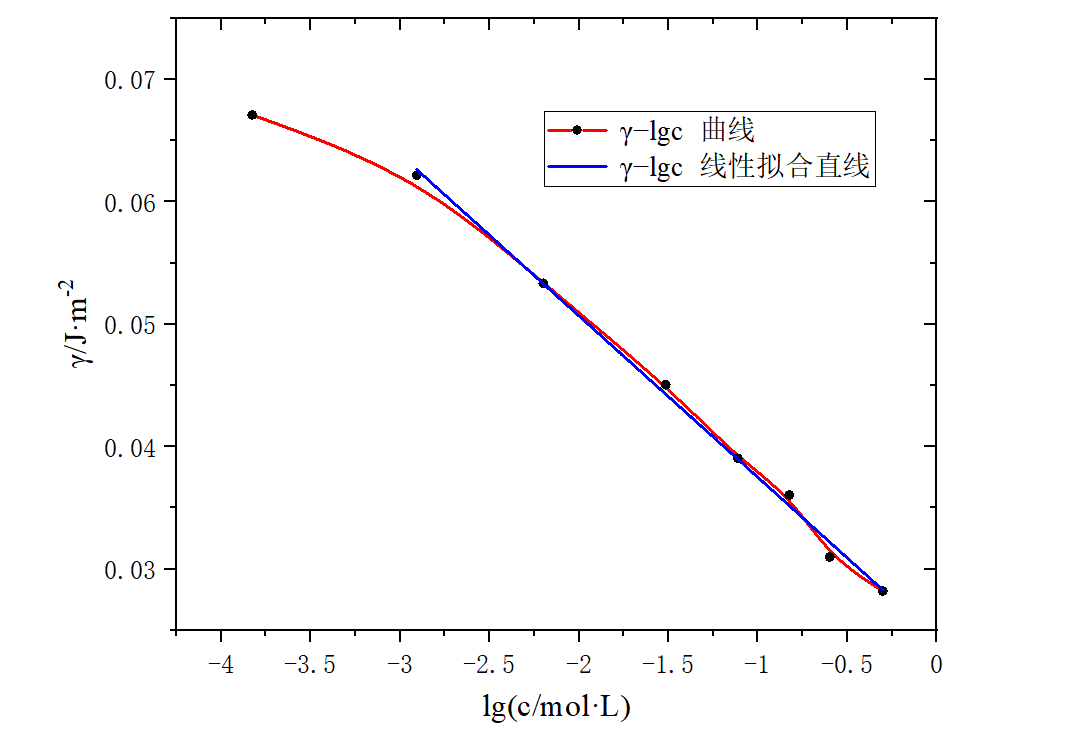
\includegraphics[width=0.8\textwidth]{3.png}
				\bicaption{正丁醇水溶液的$\gamma-{\rm ln}c$等温曲线}{Isothermal curve of $\gamma-{\rm ln}c$ of n-BuOH aqueous solution}
			\end{figure}
			\par
			根据\textbf{图3}可以看出,随着正丁醇浓度$c_{\rm BuOH}$逐渐增大${\rm ln}c$呈现下降趋势。低浓度时时$\gamma$随${\rm ln}c$的增加下降很慢,呈非线性关系;但在高于$0.0547\ \ {\rm mol\cdot L^{-1}}$的浓度范围内基本呈线性关系。\par 
			因浓度为$0.0218\ \ {\rm mol\cdot L^{-1}}$时的点明显偏离了线性曲线,故在线性拟合时舍去,取剩余的点进行线性拟合,得到的线性曲线也在\textbf{图3}中标出。线性拟合得到的直线方程为:
			$$
			\frac{\gamma}{{\rm J\cdot m^{-2}}}=(-0.01358 \pm 0.00029)\ \ {\rm ln}(\frac{c}{{\rm mol\cdot L^{-1}}})+(0.02433\pm 0.00023),\ \ R^{2}=-0.99827
			$$
			其中:
			$$
			\frac{d\gamma}{d{\rm lnc}} =  -RT\Gamma_{\infty} =(-0.01358 \pm 0.00029)\ \ {\rm J\cdot m^{-2}} 
			$$
			带入室温$T=295.65\ \ {\rm K}$,故饱和吸附量$\Gamma_{\infty}$为:
			$$
			\Gamma_{\infty}=\frac{-0.01358}{-RT} =5.52\times 10^{-6}\ \ {\rm mol\cdot m^{-2}}
			$$
			$$
			\sigma_{\Gamma_{\infty}}=\frac{0.00029}{RT}=1.18\times 10^{-7}\ \ {\rm mol\cdot m^{-2}}
			$$
			故:
			$$
			\Gamma_{\infty}=(5.52\pm 0.12)\times 10^{-6}\ \ {\rm mol\cdot m^{-2}}
			$$
			\subsubsection{最大气泡压力法计算分子吸附面积$q$与正丁醇分子实际面积$q_{c}$}
			计算每个正丁醇分子在溶液表面所占的面积:
			$$
			q=\frac{1}{\Gamma_{\infty}N_{A}}=3.01\times 10^{-19}\ \ {\rm m^{2}}=0.301\ \ {\rm nm^{2}}
			$$
			标准偏差
			$$
			\sigma_{q}=\frac{\sigma_{\Gamma_{\infty}}}{\Gamma^{2}_{\infty} N_{A}}=6.43\times 10^{-21}\ \ {\rm m^{2}}=0.064\ \ {\rm nm^{2}}
			$$
			故
			$$
			q=(3.01\pm 0.06)\times 10^{-19}\ \ {\rm m^{2}}=(0.301\pm 0.064)\ \ {\rm nm^{2}}
			$$
			\par 
			但这样的计算实际上是不精确的,因为$\Gamma$实际上是一个过剩量,即使其等于0(无吸附),表面上仍有溶质分子,因此对于较浓的溶液,在计算表面上溶质分子数时,除了吸附分子还应考虑原有分子。若$\Gamma$以$\rm mol\cdot m^{-2}$为单位,$c$以$\rm mol\cdot dm^{-3}$为单位,$q_{c}$以$\rm nm^{2}$为单位,则实际溶液浓度为$c$时的吸附量
			$$
			q_{c}=\frac{10^{18}}{\Gamma N_{A}+100\times(cN_{A})^{2/3}}
			$$
			以$c=0.740\ \ {\rm mol\cdot L^{-1}}$的正丁醇溶液为例,此时因为浓度较高,可以近似认为$\Gamma=\Gamma_{\infty}$,带入即可计算得:
			$$
			q_{c}=\frac{10^{18}}{\Gamma_{\infty} N_{A}+100\times(cN_{A})^{2/3}}=(0.26\pm 0.05)\ \ {\rm nm^{2}}
			$$
			即为该浓度下正丁醇分子在表面上的实际面积。其他浓度下的计算是类似的,但要注意,根据Langmuir吸附等温式和Gibbs吸附公式可知:
			$$
			\Gamma = \frac{\Gamma_{\infty} Kc}{1+Kc} = -\frac{c}{RT}\cdot\frac{d\gamma}{dc}
			$$
			因此,仅有当$1+Kc\approx Kc$时$\Gamma$与$ln(c)$才可近似为线性关系,当浓度较小时,$\Gamma$与$ln(c)$的关系不再是线性关系,不能简单地认为$\Gamma=\Gamma_{\infty}$。

			\vbox{}
			\subsubsection{吊片法测量正丁醇$\gamma-{\rm ln}c$曲线、饱和吸附量$\Gamma_{\infty}$、分子吸附面积$q$与正丁醇分子实际面积$q_{c}$}
			根据\textbf{3,1.4}中的数据,作出正丁醇水溶液$\gamma-{\rm ln}c$关系图散点图,并通过贝塞尔样条曲线连接各散点,形成正丁醇水溶液$\gamma-{\rm ln}c$等温曲线,如\textbf{图4}所示。
			\begin{figure}[h]
				\centering
				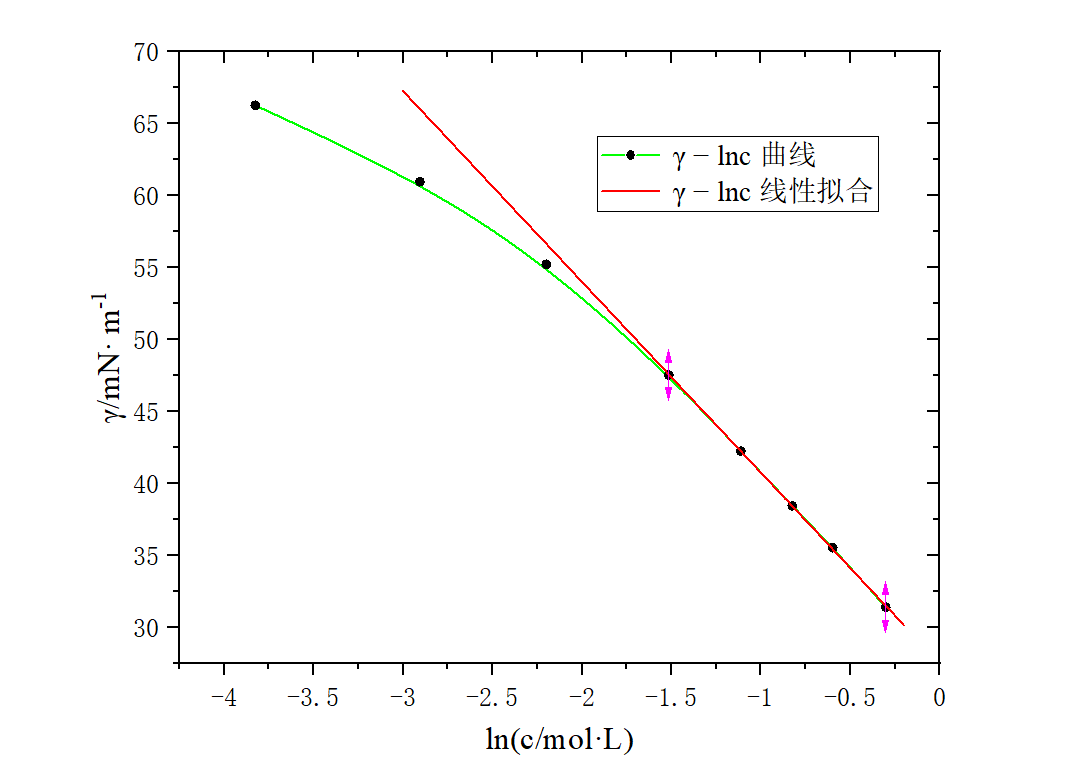
\includegraphics[width=0.80\textwidth]{4.png}
				\bicaption{吊片法测量正丁醇水溶液$\gamma-{\rm ln}c$等温曲线}{$\gamma -{\rm ln}c$ isotherm of n-BuOH aqueous solution via hanging-piece method}
			\end{figure}
			\par
			类似地,对$\gamma-{\rm ln}c$曲线近线性区的数据点(第$4\sim 8$组)进行线性拟合,所得回归直线也示于\textbf{图4}中。线性拟合得到的直线方程为:
			$$
			\frac{\gamma}{{\rm J\cdot m^{-2}}}=-(0.01324 \pm 0.00010 )\ \ {\rm ln}(\frac{c}{{\rm mol\cdot L^{-1}}})+(0.02751\pm 0.00009),\ \ R^{2}=-0.9998
			$$
			与使用最大气泡法时的计算方法相同,根据拟合直线的斜率:
			$$
			\frac{d\gamma}{d{\rm ln}c}=-(0.01324\pm 0.0001)\ \ {\rm J\cdot m^{-2}}
			$$
			代入室温$T=295.06\ \ {\rm K}$,计算饱和吸附时的饱和吸附量$\Gamma_{\infty}$值
			$$
			\Gamma_{\infty}=-\frac{1}{RT}\times\frac{d\gamma}{d{\rm ln}c}=(5.402\pm 0.04)\times10^{-6}\ \ {\rm mol\cdot m^{-2}}
			$$
			\par 
			计算每个正丁醇分子在溶液表面所占的面积
			$$
			q=\frac{1}{\Gamma_{\infty}N_{A}}=3.07\times10^{-19}\ \ {\rm m^2}=0.307\ \ {\rm nm^{2}}
			$$
			标准偏差
			$$
			\sigma_{q}=\frac{\sigma_{\Gamma_{\infty}}}{\Gamma^{2}_{\infty} N_{A}}=2.27\times10^{-21}\ \ {\rm m^{2}}=0.002\ \ {\rm nm^{2}}
			$$
			故
			$$
			q=(0.307\pm 0.002)\ \ {\rm nm^{2}}
			$$
			\par 
			对于较浓的溶液,在计算表面上溶质分子数时,除了吸附分子还应考虑原有分子。若$\Gamma$以$\rm mol\cdot m^{-2}$为单位,$c$以$\rm mol\cdot dm^{-3}$为单位,$q_{c}$以$\rm nm^{2}$为单位,则实际溶液浓度为$c$时的吸附量
			$$
			q_{c}=\frac{10^{18}}{\Gamma N_{A}+100\times(cN_{A})^{2/3}}
			$$
			以$c=0.740\ \ {\rm mol\cdot L^{-1}}$的正丁醇溶液为例,$\Gamma=\Gamma_{\infty}$,带入即可计算得:
			$$
			q_{c}=\frac{10^{18}}{\Gamma_{\infty} N_{A}+100\times(cN_{A})^{2/3}}=(0.26\pm 0.002)\ \ {\rm nm^{2}}
			$$

		\section{讨论与结论}
			\subsection{实验讨论}
			\subsubsection{吊片法测量时数值变化的原因}
			在使用吊片法测量表面张力时,试验人员发现,除了纯水测量时仪器给出的数值会相对稳定外,其他溶液测量时仪器给出的数值会随着时间的推移而发生变化。在笔者测量的浓度为$c=0.0218\ \ {\rm mol\cdot L^{-1}}$组时,这一现象还并不明显,但根据笔者观察,在后续测量更高浓度的表面张力时,测量数值会有缓慢的上升。\par
			笔者推测造成这一现象的主要原因是试剂的挥发,因为使用吊片法测量时,试剂是装在敞口表面皿中,因为水和正丁醇的挥发速率不同会导致测量过程中的浓度变化,倒是数值变化。查阅资料\citealp{dean1992lange}可知正丁醇的饱和蒸汽压大于水,因此其挥发的更快会导致溶液浓度变低,因此张力数据应当上升,与观测到的现象一致。\par
			\subsubsection{仅记录$L_{R}$数据带来的误差}
			在最大气泡压力法测量表面张力时,实验人员需要记录压力计左右两管液柱的高度差$\Delta h$,但由于需要瞬时读数,实验人员只能通过读取压力计右管液柱的高度差$\Delta h_{R}$,而压力计左管液柱的高度差$\Delta h_{L}$需要通过计算得到,即:\par
			$$
			h_{L}=h_{L,0}-(h_{R}-h_{R,0})
			$$\par
			此计算的依据为,在确定温度下水的体积不随其所处高度而变化,因此可以认为右侧水柱的高度差$\Delta h_{R}$等于左侧水柱的高度差$\Delta h_{L}$。但这么做会减少读数次数,使得单次读数的误差的翻倍,但考虑到会平行读取四组数据且度数误差相对较小,笔者认为只读取右侧液柱的高度差$\Delta h_{R}$不会对实验结果造成较大的影响。\par
			\subsubsection{其他误差来源分析}
			笔者认为本次实验中误差主要来源于以下几个方面:
			\begin{enumerate}
				\item \textbf{线性近似的忽略前提不成立}:在\textbf{3.2.2}中,笔者使用了线性近似的方法计算了饱和吸附量$\Gamma_{\infty}$,但这一近似的前提是$\Gamma$与$ln(c)$成线性关系。根据Langmuir吸附等温式和Gibbs吸附公式可知:
				$$\gamma = -RT\Gamma_{\infty}ln(Kc+1)+\Gamma_{0}$$
				当且仅当$Kc\ll 1$时:
				$$\gamma = -RT\Gamma_{\infty}ln(c)-RT\Gamma_{\infty}ln(K)+\Gamma_{0}$$\par 
				带入\textbf{3.2.2}得到的线性拟合方程中,取$\Gamma_{0} = \Gamma_{H_{2}O}$,此时$K = 21.63\ {\rm L·mol^{-1}}$,取$c=0.220\ \ {\rm mol\cdot L^{-1}}$,得到:
				$$Kc=4.76$$
				此时并不满足$Kc\ll 1$。因此线性近似的忽略前提不成立。\par
				\item \textbf{毛细管尖端未充分接触凹液面最低处,产生侧向表面张力}:由于正丁醇溶液的表面张力,毛细管尖端靠近液面的过程中,刚刚接触液面时产生液面向上隆起、“迎合”毛细管尖端的现象。此时毛细管与页面并非是相切的,这必然会引入误差。对此,应当从小试管侧下方观察,确保毛细管尖端位于实际液面最低处,与液面相切。\par
				\item \textbf{白金板表面吸附状态不同}:白金板表面的吸附能力较强,由于是不连续的进行测量,每次吸附的空气中或由待测液挥发产生的各种气体分子的量和比例不同,造成每次测定前白金板状态不同,从而引入误差。\par
			\end{enumerate}
			\subsubsection{实验的改进}
			笔者认为本实验可以改进的地方有:
			\begin{enumerate}
				\item \textbf{使用更加数字化的测量方式}:考虑到最大气泡压力法测量表面张力过程中压力计左右两端水柱高度变化速度较快,可能因测量者反应不及造成一定的读数误差,可以对该实验装置进行一定的自动化改装,例如加装传感器等以自动探测液面高度变化,从而减小实验误差。 \par
			\end{enumerate}
		\subsection{实验结论}
		\textsf{\textcolor{BrickRed}{摘\ \ 要}}\ \  \  本实验利用最大气泡压力法和吊片法,对去离子水和8个不同浓度正丁醇溶液的表面张力进行了测定,作出了正丁醇水溶液的$\gamma-{\rm ln}c$等温曲线。最大气泡压力法计算得正丁醇分子的饱和吸附量$\Gamma_{\infty}=(5.52\pm 0.12)\times 10^{-6}\ \ {\rm mol\cdot m^{-2}}$、饱和吸附下每个正丁醇分子占有的表面积$q=(0.301\pm 0.064)\ \ {\rm nm^{2}}$。当正丁醇浓度$c=0.740\ \ {\rm mol\cdot L^{-1}}$时,每个分子实际占据的面积$q_{c}=(0.26\pm 0.05)\ \ {\rm nm^{2}}$。通过吊片法计算得$\Gamma_{\infty}=(5.402\pm 0.04)\times10^{-6}\ \ {\rm mol\cdot m^{-2}}$,$q=0.307\ \ {\rm nm^{2}}$,$c=0.740\ \ {\rm mol\cdot L^{-1}}$时$q_{c}=(0.26\pm 0.002)\ \ {\rm nm^{2}}$。


		



	\vbox{}
	\section{Supporting Information}
		本实验所有的原始数据、python代码、实验报告的 LaTeX 源代码均可在\par
		 $\rm{https://github.com/wzhstat/Physical\_Chemistry\_Experiments}$找到。
\vbox{}  
%参考文献
\bibliographystyle{unsrt}
\bibliography{cite}
\end{document}